\section{Мета практикуму}
Практично ознайомитися із різними методами факторизації чисел, реалізувати методи та їх порівняння. Застосувати комбінації алгоритмів факторизації для пошуку канонічного розкладу заданого числа.

\subsection{Постановка задачі та варіант}
\begin{tabularx}{\textwidth}{X|l}
\textbf{Треба реалізувати} & \textbf{Зроблено} \\
\hline
Алгоритм перевірки числа на простоту & Імовірнісний тест Міллера-Рабіна \checkmark\\
Метод пробних ділень & Метод пробних ділень\checkmark\\
$\rho$-метод Полларда & $\rho$-метод Полларда \checkmark\\
Метод Брілхарта-Морісона/Метод Померанця & Метод Брілхарта-Морісона \checkmark\\
\end{tabularx}

\section{Хід роботи/Опис труднощів}
На початку реалізації практикуму, зробив алгоритм перевірки числа на простоту, методу пробних ділень, $\rho$-методу Полларда, адже, на мою думку вони були найпростіші. Але, на жаль, відтягував реалізацію до кінця практикуму, Брілхарт-Морісон вселяв жах у мене. Зараз його таки зробив :)

Основні труднощі виникали у піднесенні числа до певного степеня, адже числа великі та ще й не поміщалися у стандартні типи тому спробував вирішити проблему за допомогою схеми Горнера - допомогло, але для Брілхарта-Морісона уже було переповнення. Тому прийшлося шукати сторонню бібліотеку для rust.
Допомогла саме ця бібліотека(якщо так можна називати) \href{https://crates.io/crates/num-bigint}{\textit{\underline{num-bigint}}}. Саме там знайшов відповідне піднесення до степеня за модулем та без нього.

Також виникли труднощі із роботою самого Брілхарта-Морісона, бо там реалізований пошук розв'язків системи за допомогою перебору, і це давало відчутний приріст у часі роботи.
До прикладу, для числа $9172639163 = 91753*99971$ факторна база уже буде із 37 чисел, що погано піддається перебору, адже перебираю усі можливі бітові комбінації від $1$ до $(2^{37+1}-1)$, тобто від $0000..001$ до $1111..111$, де $1$ означає, що треба взяти відповідний розклад числа і додати його до загального вектора, де уже буде видно по заверешенню обходу бітового числа чи є розв'язком певна комбінація веторів за $mod 2$.
Саме на цьому числі алгоритм буде працювати $>27$ хвилин.

\begin{figure}[h]
			\center{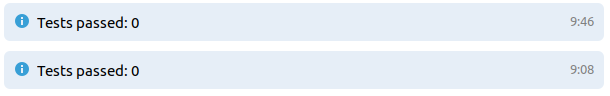
\includegraphics[scale = 0.45]{time_test_1}}
			\caption{Приклад орієнтовоного часу роботи Брілхарта-Морісона для великих чисел.}
			\label{fig:image}
		\end{figure}

\section{Результати дослідження}
У результаті маємо, що:
\begin{enumerate}
\item Імовірнісний тест Міллера-Рабіна --- дуже ефективниий алгоритм перевірки на простоту за допомогою означення \textit{псевдопростоти за Ойлером}, що дає нам ймовірність помилки $\dfrac{1}{4^{k}}$(краще чим у Соловея-Штрассена --- $\dfrac{1}{2^{k}}$, де $k - $кількість повторень алгоритму), але треба звернути увагу на ефективну реалізацію піднесення до степеня за модулем.
\item Алгоритм пробних ділень --- є ефективним для дуже малих чисел, до прикладу, для $\leqslant47$. Адже він працює за допомогою перебору чисел до $\sqrt{n}, n -$ вхідне число, що не є ефективним для набагато більших чисел.
\item $\rho$-метод Полларда --- є дуже ефективним для розкладу чисел, де прості дільники знаходяться не далеко від одного, наприклад, як $8633 = 97*87$. Адже цей алгоритм побудований за допомогою обчислення орбіти, яка у свою чергу обчислюється псевдорандомними функціями типу $x^{2}+1$..
\item Метод Брілхарта-Морісона --- належить зовсім іншому класу алгоритмів, адже побудований на факторній базі, яка дозволяє розкладати дуже великі числа (але у мене не вийшло ефективно його реалізувати :( ). Саме тут критичним є перебір усіх можливих варіантів розв'язку, дуже впливає на сам час роботи.
\end{enumerate}

\begin{figure}[h]
			\center{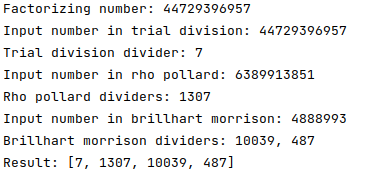
\includegraphics[scale = 0.5]{example1}}
			\caption{Приклад факторизації усіма алгоритмами числа 44729396957.}
			\label{fig:image}
		\end{figure}
		
\begin{figure}[h]
			\center{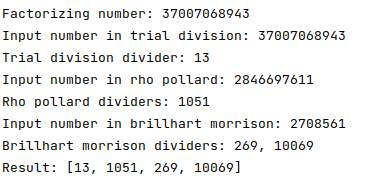
\includegraphics[scale = 0.5]{example2}}
			\caption{Приклад факторизації усіма алгоритмами числа 37007068943.}
			\label{fig:image}
		\end{figure}

\vspace{40mm}
\section{Продуктивність}
\vspace{3mm}
Після обрахунків вийшло наступне:

\begin{tabularx}{\textwidth}{||l|c|l||}
  \textbf{Числа} & \textbf{$\rho$-метод Полларда} & \textbf{Брілхарт Морісон} \\
9172639163 & 549.089µs & $\geqslant27$min\\
9172639163862795 & 1.862472ms & ---\\
8627969789 & 514.899µs & ---\\
8937716743 & 875.838µs & ---\\
278874899 & 350.56µs & ---\\
99400891 & 180.081µs & ---\\
116381389 & 195.414µs & ---\\
4252083239 & 477.629µs & ---\\
6633776623 & 272.11µs & ---\\
227349247 & 138.315µs & ---\\
3568572617 & 327.826µs & ---\\
25511 & 48.185µs & 10.984851ms\\
3973573 & 90.012µs & 28.210255ms\\
10528813 & 202.815µs & 42.002997ms\\
4248311 & 146.742µs & 28.151853ms\\
10252159 & 93.764µs & 66.936453ms\\
5746331 & 107.961µs & 35.10992ms\\
2708561 & 27.814µs & 62.165807ms\\
10169711 & 152.216µs & 32.830382ms\\
4888993 & 85.48µs & 27.730359ms\\
12404297 & 107.104µs & 35.126146ms\\
11587117 & 86.53µs & 79.249916737s\\
\end{tabularx}

\vspace{5mm}
\textbf{Оцінка продуктивності}:
\begin{enumerate}
\item $\rho$-метод Полларда --- працює для $\leqslant16$ значних чисел, для 17 уже треба чекати.
\item Метод Брілхарта-Морісона --- на маленьких числах застосовується, що із двома великими дільниками добре, а от із 4 - уже виникають проблеми.
Погано працює уже для $>11587117$.
\end{enumerate} 

\section{Висновки}
За допомогою реалізації практикуму ''Пошук канонiчного розкладу великого числа,
використовуючи вiдомi методи факторизацiї'', дізнався на практиці, як працюють алгоритми факторизації. $\rho$-метод Полларда вийшов досить ефективним, працює навіть караще чим Брілхарта Морісона. Рекомендую при реалізації цих алгоритмів самотужки заздалегідь визначитися із тим, як: реалізувати обчислення елементарних операцій, взяття по модулю, піднесення до степеня, зберігання великих чисел. Бо, як переконався на власному досвіді, все вищезазначене дуже сильно впливає на ефективність реалізації.
А от криптографічних цілях, на мою думку, краще реалізувати алгоритм Померанця та інші ефективніші алгоритми базовані на факторній базі.

		

	




